\lfoot{Autor: Raphael Simsek}
\subsection{Analyse und Verbesserung des Fahrstils}

Leider kann nicht immer der Fahrlehrer einem Fahrschüler einen nachhaltigen oder wünschenswerten Fahrstil näher bringen, da dies oft auch ein zeitintensiver Prozess ist. Zu diesem Zweck machte man sich Gedanken wie man diese Situation verbessern kann.

Vor der Antragstellung wurde überlegt, ob es bereits bekannte Systeme gibt, um seinen Fahrstil nachhaltig zu verbessern. Man fand dabei heraus, dass es bereits in vielen anderen Bereichen Apps gibt, welche sich das \textit{Sharing}-Prinzip zu Nutze gemacht haben und so äußerst bekannt geworden sind. Eines der bekanntesten österreichischen Beispiele ist das, stetig erweiterte, App-System von Runtastic. \cite{SIMR.CH1-Fahrstil-Analyse.BusinessplanRuntastic}
Nur in Bezug auf das Autofahren konnte kein System, das dieses Prinzip verfolgt, gefunden werden.

\comment{MELD:Was hat das alles konkret mit Analyse und Verbesserung des Fahrstiles zu tun? - Element der Peer-Pressure erklärt und integriert, so besser?}
Zu Beginn des Diplomprojektes gab es also keine Möglichkeiten für verbesserungswillige Autofahrer ihren Fahrstil zu verbessern und dies dann sogar zu teilen. Das Teilen der Fahrstilanalyse trägt aufgrund des \textit{Peer-Pressure}-Effekts dazu bei, dass die Nutzer ihren Fahrstil verbessern, da Sie andere Nutzer überbieten möchten. So versuchen sich die Fahrer dadurch also stetig zu verbessern.
Dies hat unsere Marktumfeldanalyse ergeben, wobei uns besonders auffiel, dass eine Analyse-Funktion für die nachhaltige Verbesserung des Fahrstils nötig wäre. Es wurde für diese Analyse evaluiert, welche Funktionalitäten am wichtigsten sind, wobei diese auch innerhalb der Diplomarbeit realisierbar sein sollten. 
\newline

Eine Analyse des Fahrstils, nach Parametern der Fahrgastbequemlichkeit, ist gar nur bei Sportwagen und Fahrzeugen, die für den Rennbetrieb gedacht sind, verbaut. Hierbei ist anzumerken, dass bei derartigen Fahrzeugen die Funktionalität nicht für das frühzeitige Verbessern des Fahrstils eines Fahrers verwendet wird, sondern für die Optimierung von Rundenzeiten auf einer Rennstrecke oder schier für das Ausreizen des Möglichen.

\begin{figure}[!htb]\centering
	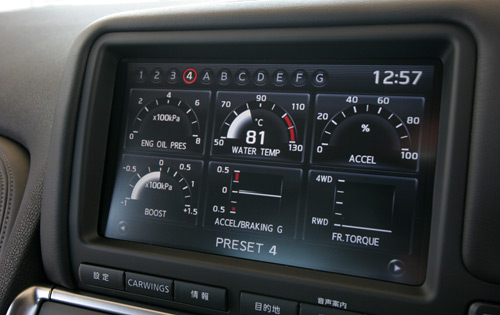
\includegraphics[width=0.6\textwidth]{images/gtrMultifunc}
	\caption{bisherige Analyse Möglichkeiten bei einem Nissan GT-R (R35) \cite{SIMR.CH1-Fahrstil-Analyse.GTRMultifunc}}\label{Fig:imgGTR}
\end{figure}

\newpage
Der bisherige Schaltvorschlag in einem Auto ist, insbesondere bei kostengünstigeren Fahrzeugen, oft äußerst simpel gehalten, wobei ab einer gewissen Drehzahl die darauffolgenden Gänge vorgeschlagen werden oder nur auf den Normzyklus optimiert wird. \cite{SIMR.CH1-Fahrstil-Analyse.Schaltempfehlung} Der Motorwirkungsgrad nach dem Carnot-Prozess, wird dabei aber kaum verwendet. \todo{Insert Carnot-Prozess description, add efficiency graph}\cite{SIMR.CH1-Fahrstil-Analyse.CarnotWirkungsgrad} Genauere Ausführungen zu diesem Thema finden Sie im Kaptiel Thermodynamik \hyperlink{subsubsection.2.1.2}{mehr}. \todo{fix inter-chapter reference}

Eine Live-Messung von CO2 Werten während der Fahrt ist momentan eine Schätzung, welche durch die Fahrzeughersteller aufgrund der OBD-II Daten durchgeführt und bei sehr wenigen Modellen als Zusatz angezeigt wird. Echte Grenzwerte oder gar eine Analysefunktionalität gibt es in dieser Hinsicht aber nicht. Die CO2 Werte werden in Zukunft noch weitaus relevanter, weil, wie mein Kollege im folgenden Kapitel ausführlich beschreibt, bis 2020 versucht wird einen Durschnittsaustoss von 95 g/km zu erzielen. \cite{SIMR.CH1-Fahrstil_Analyse.EUVerordCO2}

Weil aber besonders Fahranfänger und Fahrer die eben genannte Analysefunktionalität möglicherweise gerne nutzen würden, wurde ebenfalls evaluiert ob es diese Möglichkeiten durch Zubehör bereits gibt.

Bei der Evaluierung wurde ein Projekt entdeckt, welches die gelieferten Daten nur live per Computer auslesbar macht, die Programmierung ist dabei so anders dass man dies nicht auf Android portieren könnte. Das Projekt ist außerdem weitaus teurer als angedacht (Low Budget CarPC: €300-350,-, gewünschtes Budget: < €100,-) Daher wurden Überlegungen angestellt, wie man die Idee eines solchen Projektes massentauglicher machen kann und dabei trotz des niedrigeren Preises dem Nutzer ein wünschenswertes Erlebnis bieten kann. \cite{SIMR.CH1-Fahrstil-Analyse.LowBudgetCarPC} Dieses Projekt hat uns also geholfen in der Defintionsphase des Projektes Anpassungen vorzunehmen, da es bereits einen Maßstab gab, was im Bereich des Möglichen liegt.

Die Möglichkeit einer Analyse konnte aber bei der Evaluierung bei keiner der konkurrierenden Echtzeit-Anzeigen (wie. z.B. Torque Pro \cite{SIMR.CH1-Fahrstil-Analyse.TorquePro}) erkannt werden. 

\begin{figure}[!htb]\centering
	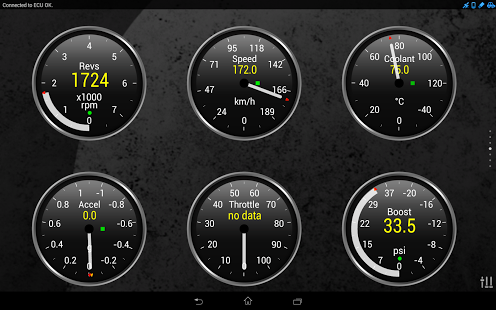
\includegraphics[width=0.6\textwidth]{images/torquePro}
	\caption{Möglichkeiten mit der kostenpflichtigen Torque Pro App und der OBD Schnittstelle \cite{SIMR.CH1-Fahrstil-Analyse.TorquePro}}\label{Fig:imgGTR}
\end{figure}

Gerade diese Funktionalität würde aber von Fahranfängern benötigt werden um frühzeitig und selbstständig Fehler ihres Fahrstils zu erkennen und auszubessern zu können. Insbesondere konnten wir, unter anderem anhand unserer Erfahrungen, feststellen, dass das Schalten und das gleichmäßige und verbrauchsarme Fahren für viele Fahranfänger eine Herausforderung darstellt. Durch eine Analyse Funktion könnten motivierte Fahranfänger Anfangsschwieriegkeiten schneller ablegen und die schlechten Angewohnheiten würden sich nicht im  Gedächtnis eines Fahranfängers verankern, sondern es würden sich nur positive Charakteristika gemerkt werden. \comment{JOSC: Definiere bitte positive und schlechte Angewohnheiten oder formulier um - so?} 

Eine Analysefunktion in Form einer Webapplikation ist also insbesondere für die Lernkurve bei einem noch ungeübten Kraftfahrzeug-Lenker von großem Vorteil, da diese oft noch nach dem Erhalt des Führerscheins unsicher bezüglich ihres Fahrstils sind und des öfteren wiederholt die selben, genannten, Fehler unbemerkt begehen.

Andererseits kann solch eine Funktionalität auch von großer Hilfe als lernunterstützendes Medium sein, da momentan ein Fahrschüler nach seiner Fahrstunde nur ein subjektives Feedback seines Fahrlehrers bekommt. Wie ließe sich eine solche Lernunterstützung also umsetzen?
Man könnte dem Fahrschüler am Ende der Fahrstunde eine faktenbasierte Übersicht über seine Leistung während der Fahrstunde geben, welche er dann auch mitnehmen kann. Mit dieser Information kann sich der Fahrschüler ohne Fahrlehrer mit der App selbst im Auto auf abgesperrtem Grund verbessern um sich so auf die nächste Fahrstunde vorzubereiten.

Ein geübter, umweltfreundlicher Fahrer könnte mit der passenden Analysefunktion auch den produzierten CO2 Ausstoß messen und so seinen Bleifuß besser regulieren.
\clearpage % DO NOT REMOVE
